\chapter{Construcción Paralela sujeta a $RG$}
\label{champ:PBSGR}
\bigskip
\barra
\bigskip
En este capítulo se describe la implementación paralela de los algoritmos descritos en el capítulo \ref{champ:BSGR} para la creación de redes porosas sujetas a Restricciones Geométricas. Las implementaciones paralelas trabajan sobre el modelo  de memoria compartida, donde varios hilos cooperan en la construcción de una red porosa válida siguiendo los principales pasos de los algoritmo presentados en el capítulo anterior. El primer paso para las dos soluciones paralelas es la distribución espacial de la red entre los hilos después viene la inicalizaci\'on y por \'ultimo la generación una red porosa v\'alida.

\section{Distribución de la red porosa}
\label{sec:pdistribution}
En este paso una red porosa es dividida en $N$ subredes donde $N$ es el número de hilos a utilizar. El objetivo de este paso es dividir la red en $N$ subredes las cuales deben mantener una estructura lo más parecida a un cubo, para lograr esto la red se divide a lo largo de los tres ejes $x$,$y$ y $z$ respectivamente cada eje se dividirá $a$, $b$, y $c$ partes. Se debe cumplir que el producto de  $a$, $b$, y $c$ es igual a $N$. El tamaño de cada subred esta definido por $L_x \cdot L_y \cdot L_z$, como se puede observar en la Figura \ref{fig:distribution}. Si por ejemplo tomamos $N=4$, la configuración generada ser\'ia $a=1,b=2,c=2$, mientras que para $N=45$ la configuración generada ser\'ia $3,3,5$, y para  $N = 27$ la configuración generada ser\'ia $3,3,3$ que representa la raíz cubica de 27. La mejor distribución se da cuando $a$, $b$, y $c$ corresponden a la raíz cubica de $N$; de esta forma las subredes generadas adoptan la una estructura cúbica que ayuda a que la distribución de los poros sea equitativa a lo largo de los ejes $x$, $y$ y $z$ de cada subred. En la Figura \ref{fig:particionamiento} se muestran algunos ejemplos de particionamiento.\\

\begin{figure}[hbtp]
\centering
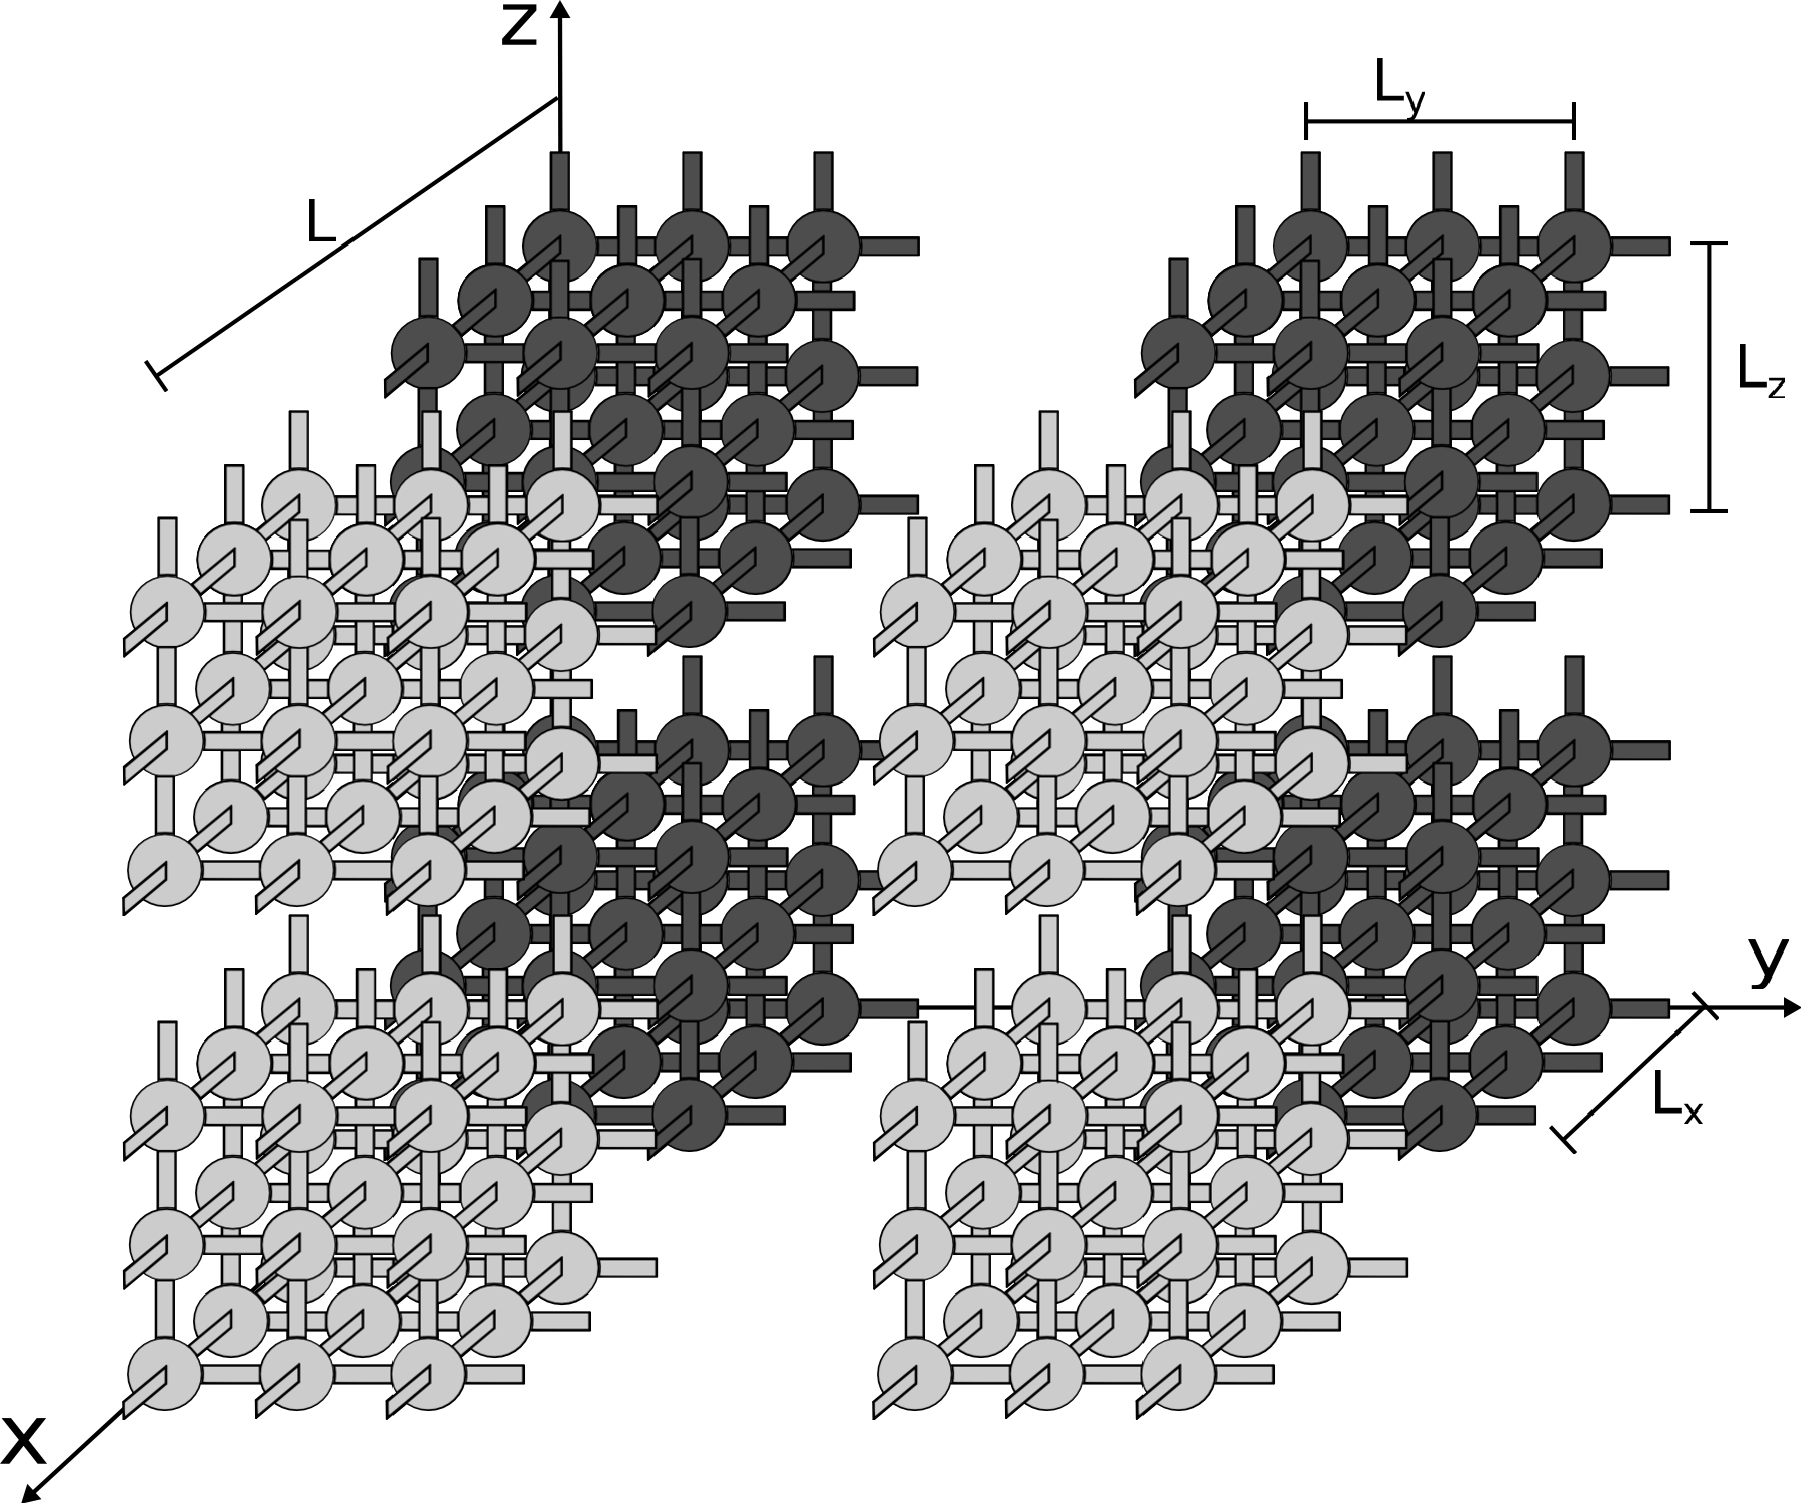
\includegraphics[width=3.5in]{img/distribucion.pdf}
\caption{Red porosa dividida en ocho subredes; $N=2\cdot2\cdot2$}
\label{fig:distribution}
\end{figure}

\begin{figure}[hbtp]
\centering
\begin{tabular}{cc}
\subfloat[$(1,2,2)$]{
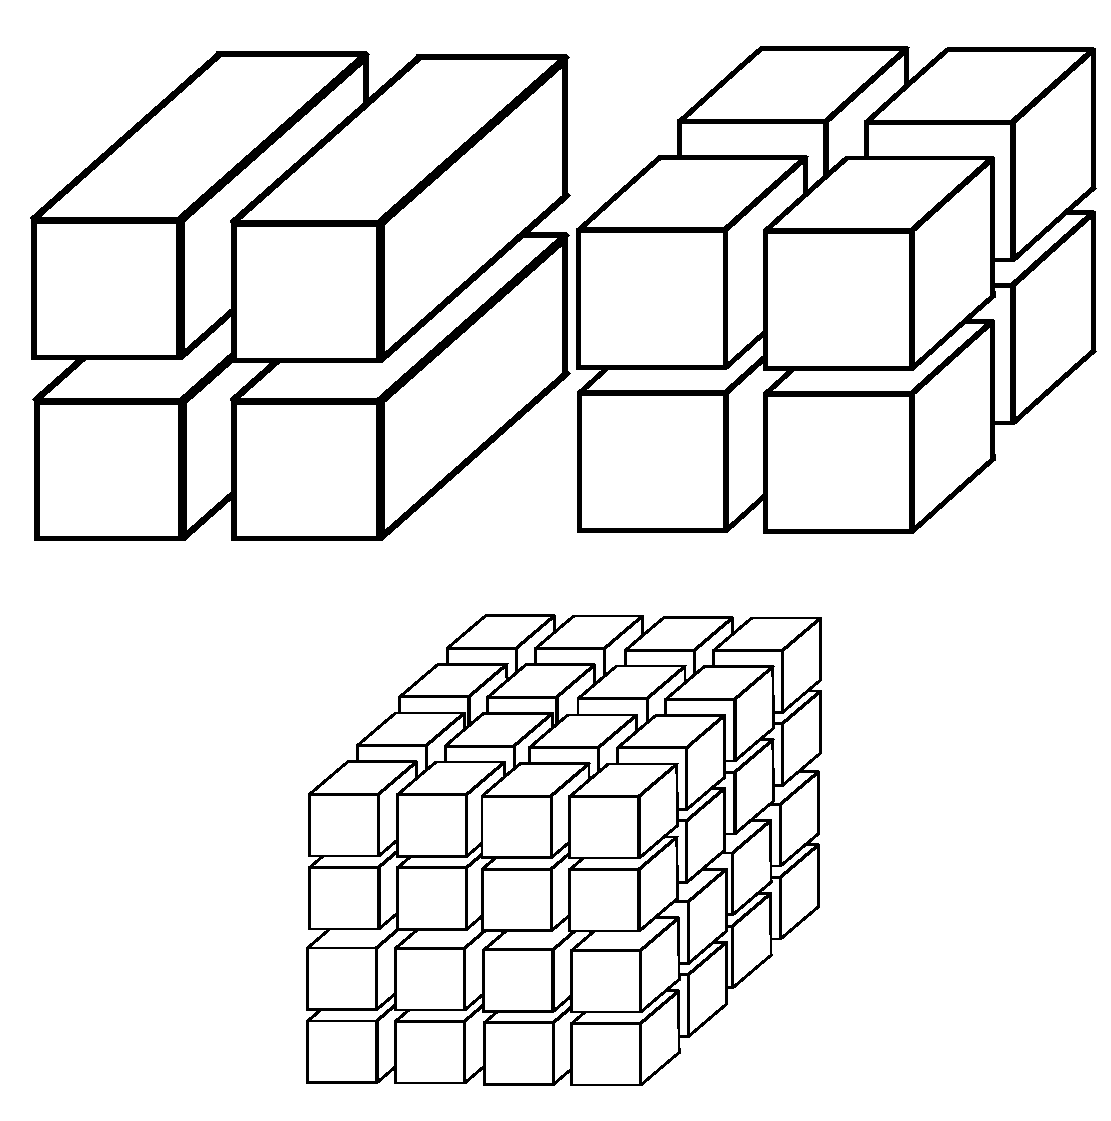
\includegraphics[width=2.0in, viewport=15 265 273 515,clip]
 {img/particionamiento.pdf}
\label{fig:part4}}
& \subfloat[$(2,2,2)$]{
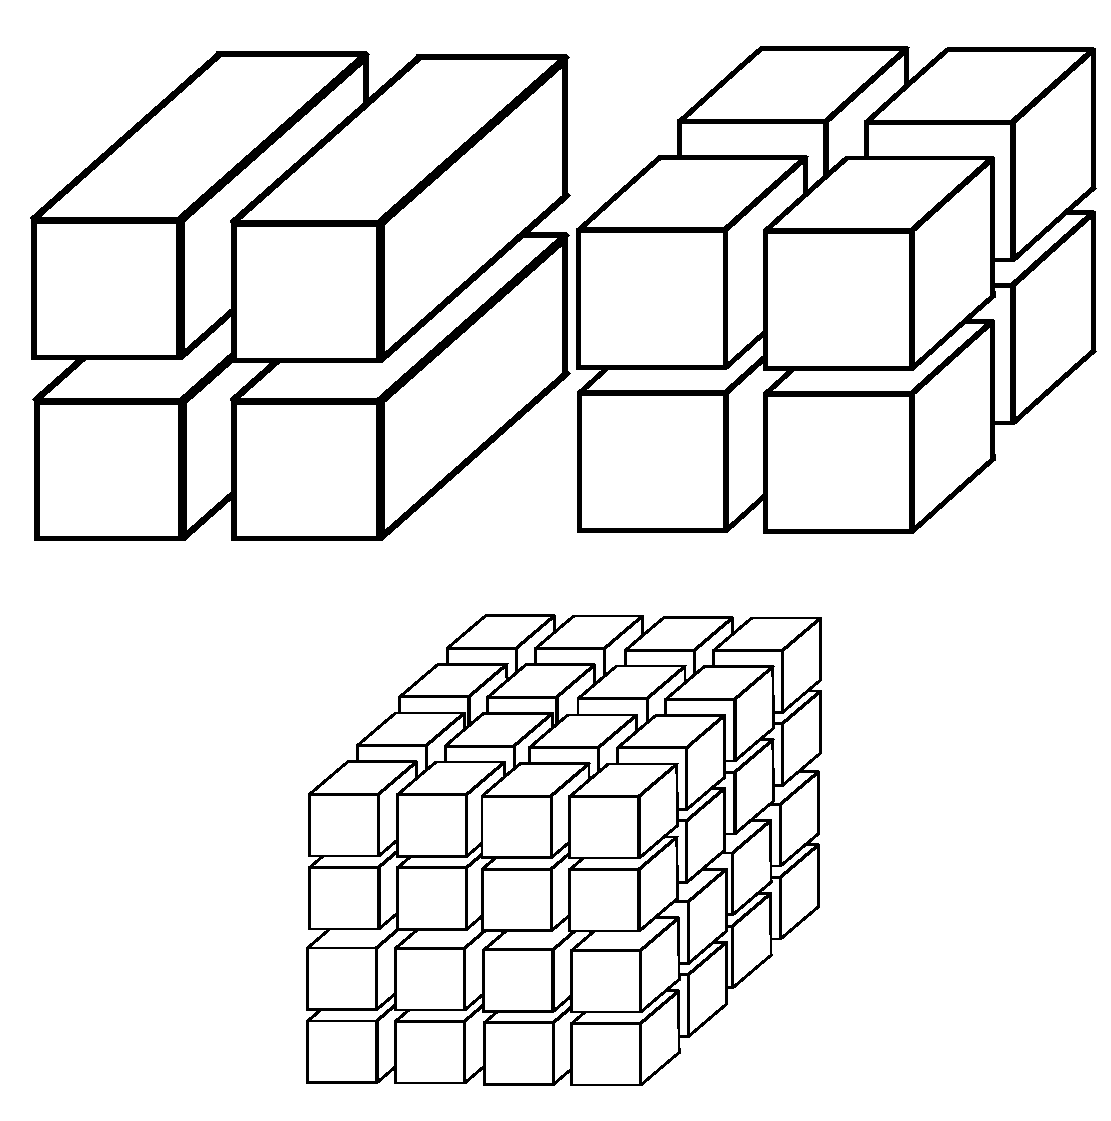
\includegraphics[width=2.0in, viewport=275 265 525 515,clip] {img/particionamiento.pdf}
\label{fig:part8}}\\

\multicolumn{2}{c}{
\subfloat[$(4,4,4)$]{
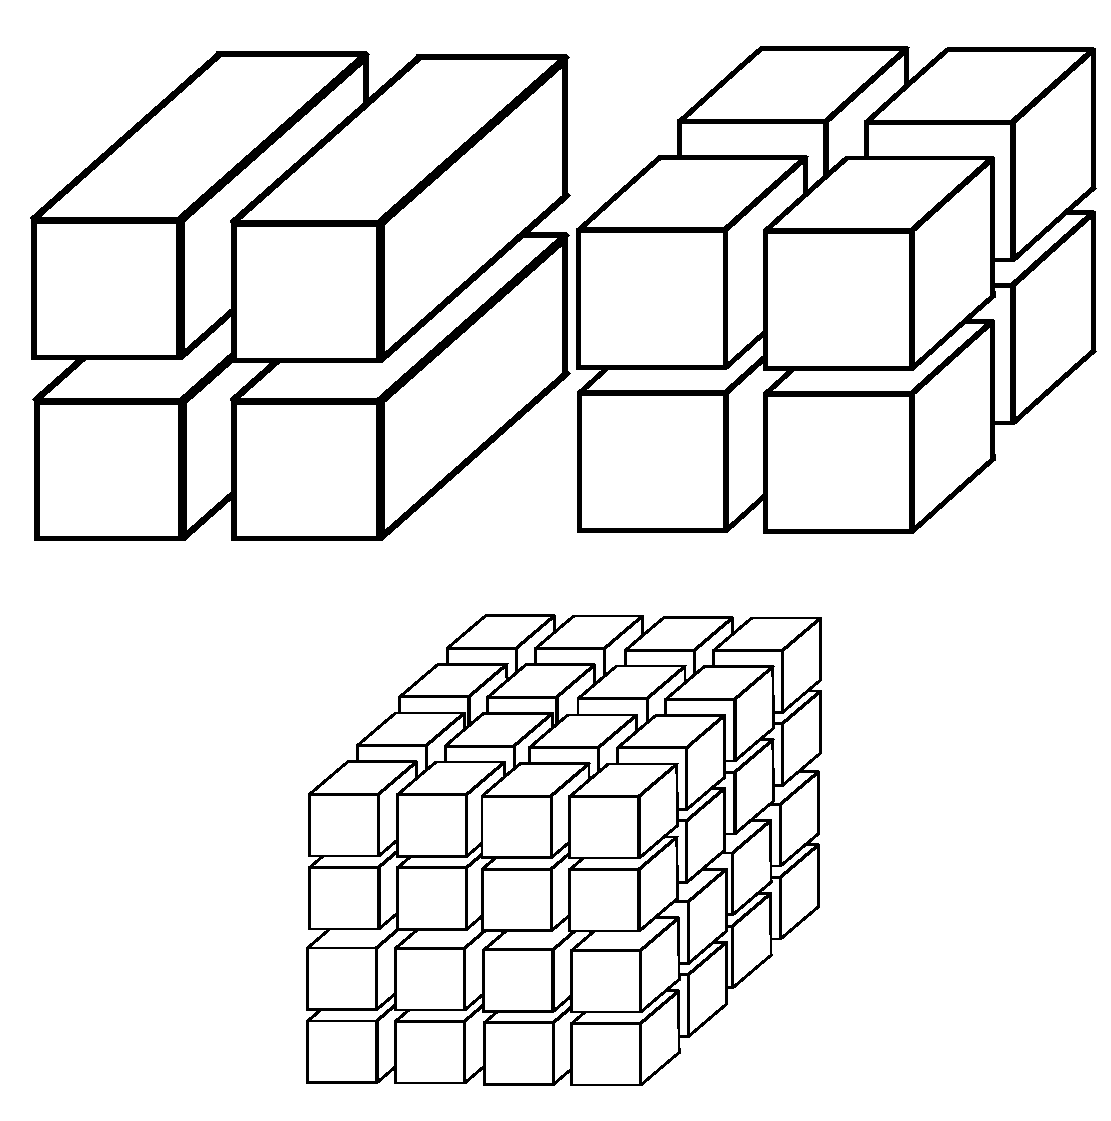
\includegraphics[width=2.0in, viewport=145 0 395 250,clip] {img/particionamiento.pdf}
\label{fig:part64}}
}
\end{tabular}

\caption{Distribución de la Red para (a) 4 hilos, (b) 8 hilos, and (c) 64 hilos}
\label{fig:particionamiento}
\end{figure}

\section{Solución Paralela Aleatoria}

%\subsection{Inicialización}
%\label{subsec:painit}

%Una vez que la red porosa fue distribuida entre los $N$ hilos a utilizar utilizando el algoritmo descrito en la sección anterior, es decir la red porosa se dividió en $N$ suredes donde cada subred tiene un tamaño $L_x \cdot L_y \cdot L_z$ tal y como se muestra en la Figura \ref{fig:distribution}. De esta forma cada hilo trabajara de forma independiente sin necesidad de sincronizarse durante el proceso de inicalización, cada hilo insertara de forma aleatoria en su subred $L_x \cdot L_y \cdot L_z$ sitios hasta rellenar por completo la red, una vez que la red esta completamente inicializada con sitios a cada sitio se le asignara únicamente tres enlaces(izquierdo, trasero y superior) esto para evitar la sincronización entre los hilos.

Una vez que la red porosa fue distribuida entre los $N$ hilos utilizando el algoritmo descrito en la sección anterior, cada hilo trabajara de forma independiente en una subred de tamaño $L_x \cdot L_y \cdot L_z$ tal y como se muestra en la Figura \ref{fig:distribution} sin necesidad de sincronizarse durante el proceso de inicalización.

Cada hilo inserta de forma aleatoria en su subred $L_x \cdot L_y \cdot L_z$ sitios hasta rellenar por completo la red, una vez que la red esta completamente inicializada con sitios a cada sitio se le asignara únicamente tres enlaces(izquierdo, trasero y superior) esto para evitar la sincronización entre los hilos.

\subsection{Generación de una Red Porosa Válida}
\label{subsec:pavalid}

\subsection{Mejoramiento de la isotropía}
\label{subsec:paisotropy}

\section{Solución Paralela Híbrida}
\subsection{Inicialización}
\label{subsec:pinit}
Los hilos trabajan en subredes diferentes. por cada hilo, tal y como en la solución propuesta en el capítulo anterior se generan las listas ordenadas $L_S$ y $L_B$. $L_S$ contiene $L_x \cdot L_y \cdot L_z$ tamaños de sitos ordenados de forma descendente, y $L_B$ contiene $3\cdot L_x \cdot L_y \cdot L_z$ tamaños de enlaces ordenados también de forma descendente. La sincronización entre los hilos no es necesaria para el uso o modificación de las listas $L_S$, $L_{SC}$ and $L_B$ porque estas listas son locales a cada hilo.

\subsection{Sembrado de Clusters}
\label{subsec:pseeding}
Por cada hilo, el número de semillas corresponde a $NClusters/N$. Cada semilla es insertada en una posición aleatoria en su respectiva subred. Los demás elementos en $L_S$ son tomados uno por uno para cubrir la semilla y formar un cluster, tal y como se explica en el capítulo anterior. La posición aleatoria en la cual se asignara la semilla en la subred es generada de tal forma que no puede ser asignada en las caras externas de la subred. Durante el sembrado todos los hilos se sincronizan a través de una $barrera$ después de que cada uno complete un cluster, entonces el origen $(x, y, z)$ se cambia  de forma aleatoria a lo largo de los ejes $x$,$y$ y $z$ en rango que esta entre $0$ to $L-1$. El cambio de origen se hace con el propósito de que los hilos puedan trabajar en subredes independientes y diferentes de la red porosa.\\

El origen de la red porosa esta inicialmente en $(0,0,0)$, como se muestra en la Figura \ref{fig:origin1}, si movemos el origen a $(0,2,0)$, esto causaría que las áreas de trabajo(subredes) de cada hilo cambien como se muestra en la Figura \ref{fig:origin2}, las nuevas áreas de trabajo se resaltan en color azul y naranja.\\

\begin{figure}[hbtp]
\centering
\begin{tabular}{c}

\subfloat[Distribución inicial del espacio]{
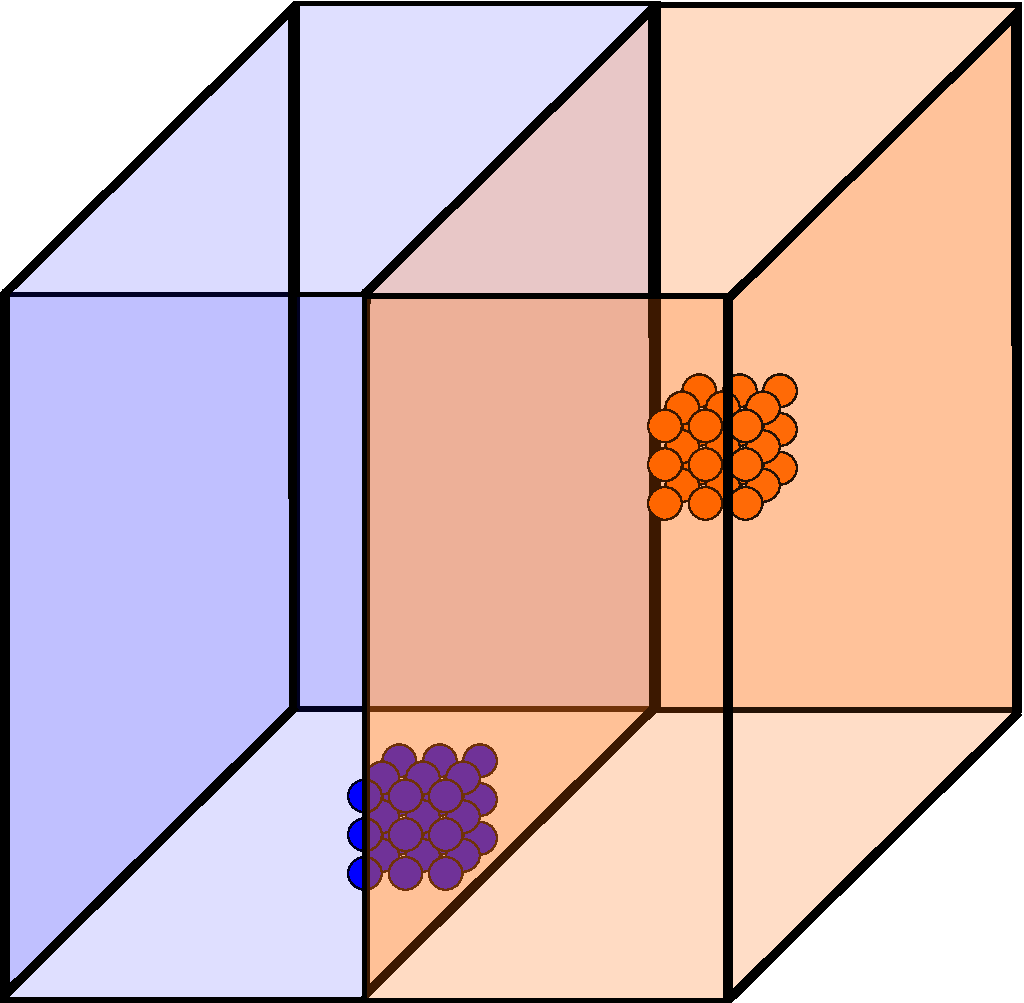
\includegraphics[width=4.0in]{img/origin1.pdf}
\label{fig:origin1}}\\

\subfloat[Distribución posterior del espacio]{
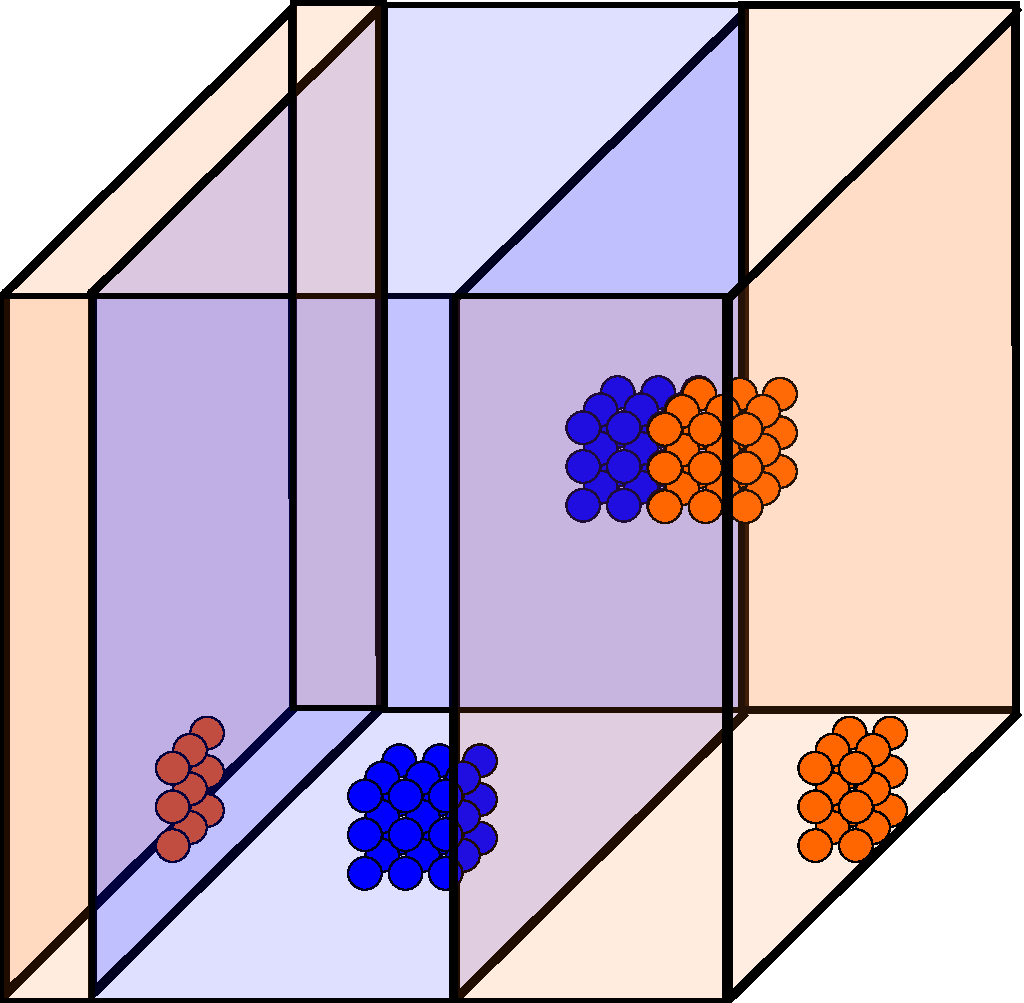
\includegraphics[width=4.0in] {img/origin2.pdf}
\label{fig:origin2}}

\end{tabular}

\caption{(a) Origen en ($0,0,0$) y (b) cambio de origen a ($0,2,0$)}
\label{fig:origin}
\end{figure}

Después de completar el sembrado de clusters, el origen de la red es trasladado a ($0, 0, 0$) de manera que cada hilo, comienza a trabajar en su subred inicial. El siguiente paso consiste en rellenar su actual subred con los sitios restantes en su lista $L_S$; sin embargo en este momento el número de sitios en las listas $L_S$ de cada hilo son diferentes. Puede que para algunos hilos los sitios que tienen en sus listas $L_S$ no sean suficientes para rellenar su subred, mientras que otros pueden tener sitios de sobra en sus listas $L_S$ de los requeridos para rellenar su subred. Para solucionar el problema anterior los elementos de las listas $L_S$   requieren ser distribuidos entre los hilos.\\

Los pasos necesarios para distribuir los elementos de las listas $L_S$ se presentan en el Algoritmo \ref{alg:sitesdist} el cual es una versión simplificada del algoritmo presentado en \cite{ref11} para la distribución de carga.\\

Por cada hilo se tiene, identificador del hilo ($id$), el número $M[id]$ de sitios requeridos el cual depende de: el tamaño de la subred $SNS[id]$ ($SNS[id] = L_x \cdot L_y \cdot L_z$), el número de sitios que ya han sido insertados en la subred $SI[id]$, y el número de sitios en su lista $AL_S[id]$, denotado por $Size(L_S[id])$. En el algoritmo el arreglo $M$ su contexto es global por lo cual es es una variable compartidas.\\

La primera etapa consiste en el calculo del número de sitios requeridos; cada hilo calcula $M[id]$ como se indica en la linea 1 del Algoritmo \ref{alg:sitesdist}. En el segundo paso, los hilos que tienen $M[id]<0$, que indica que tienen sitios de sobra y es por eso que insertan su $id$ en la lista compartida de Hilos Pesados denotada por $HT$,(line 4), esta inserción se hace a través de exclusión mutua entre los hilos (lineas 2-6). Después todos los hilos se sincronizan mediante un mecanismo de barrera (linea 7). Esta barrera hace que los hilos con $M[id]>0$ (con sitios faltantes) esperen a que la lista $HT$ sea inicializada por los demás hilos. En el último paso, los hilos con $M[id] > 0$ trabajan utilizando exclusión mutua (lineas 9-23) para tomar sus sitios faltantes de las listas $L_S$ de los hilos en $HT$. Cuando un hilo $id$ toma los sitios de otro hilo $k$ en $HT$ (lineas 13 y 17), los nuevos valores $M[id]$ y $M[k]$ se actualizan, como se muestra en las lineas 14, 15, 18 y 19. En caso de que un hilo en $HT$ había dado todos sus hilos sobrantes, este es removido de la lista $HT$ (linea 20).\\

Una vez que la distribución de los sitios es completada, cada hilo hace crecer su primer cluster generado hasta rellenar por completo su subred y su lista $L_S$ esta vacía.
 
%\newcommand{\INDSTATE}[1][1]{\State\hspace{#1\algorithmicindent}}
\begin{algorithm}
\caption{Redistribución de los sitos entre los hilos}\label{alg:sitesdist}
\begin{algorithmic}[1]
%\algblock[Name]{ompcritical}{End}
\algblockdefx[NAME]{ompcritical}{eompcritical}
    {\textbf{omp critical}}
    {\textbf{end omp critical}}
    
\Require $M$: Arreglo compartido
\Require $HT$: Lista compartida de hilos pesados
\Require $id$: Identificador del hilo
\State $M[id]=SNS[id]-SI[id]-Size(L_S[id])$
\If{$M[id]<0$}
	\ompcritical
		\State \Call{InsertId}{$id,HT$}
	\eompcritical
\EndIf
\State \textbf{omp barrier}
\If{$M[id]>0$}
	\ompcritical
		\While{$M[id] > 0$}
			\State $k=getFirst(HT)$
			\If{$M[id] < |M[k]| $}
				\State \Call{MoveNSites}{$M[id],L_S[id],L_S[k]$}
				\State $M[k]=M[k]+M[id]$
				\State $M[id]=0$
			\Else
				\State \Call{MoveNSites}{$M[k],L_S[id],L_S[k]$}
				\State $M[k]=0$
				\State $M[id]=M[id]+M[k]$
				\State \Call{RemoveId}{$k,HT$}	
			\EndIf
		\EndWhile
	\eompcritical
\EndIf
\end{algorithmic}
\end{algorithm}

\subsection{Asignación de Enlaces}
\label{subsec:pbond}
En la sección anterior, cada hilo mantuvo su lista $L_{SC}$, la cual contiene las posiciones de los sitios insertados durante el sembrado y rellenado de red porosa, tal y como se hace en la solución básica. La listas $L_{SC}$ de cada hilo contienen las posiciones en las cuales se insertaron los sitios a lo largo de la red porosa; sin embargo sus los elementos de la lista $L_SC$ están dispersos en la red porosa.\\

Debido a las acciones realizadas en la sección anterior las listas $L_{SC}$ se pueden estar en desbalance por lo que es necesario distribuir los elementos entre los hilos. Para distribuir los elementos de las listas $L_{SC}$ se utiliza el mismo algoritmo que de la sección anterior (Algoritmo \ref{alg:sitesdist}), con dos cambios, el primero es el cambio en todo el algoritmo de $L_S$ por $L_{SC}$ y el segundo es cambiar la linea 1 por $M[id]=SNS[id]-Size(L_{SC}[id])$.\\

Una vez que las listas están balanceadas, cada hilo, toma las posiciones de los sitos una a uno de la lista $L_SC$ y conecta los tres correspondientes enlaces al sitio (izquierdo, trasero y superior). Cada conexión entre sitio y enlace debe cumplir con el $PC$ y las $RG$, siguiendo el mismo procedimiento descrito en la sección \ref{subsec:sbonds}. Cada sitios es conectado a solo tres enlaces porque, como se define en el Capítulo \ref{champ:intro}, un sitio tiene tres enlaces propios mientras que los otros tres enlaces son compartidos con los sitios vecinos. Lo anterior se hace para evitar la sincronización entre los hilos que posiblemente se necesitara al conectar los enlaces compartidos (derecho, frontal e inferior). Al finalizar este paso se obtiene una red porosa con violaciones al $PC$ y a las $RG$.

\subsection{Generación de una red porosa válida}
\label{subsec:pvalid}
Para que la red creada a partir de los pasos descritos en las secciones anteriores de este capítulo sea válida en términos del $PC$ y de las $RG$, es necesario aplicar una serie de $MCs$ para eliminar por completo las violaciones. Por cada intercambio de sitios o enlaces durante un $MCs$ el $PC$ y las $RG$ deben ser respetadas.\\

De igual manera los $MCs$ se realizaran paralela a través de hilos los cuales trabajan de manera independiente en distintas subredes, los pasos para el intercambio de poros son los siguientes: 

\begin{enumerate}
\item La red porosa es dividida en $2N$ subredes utilizando el algoritmo descrito en la Sección \ref{sec:pdistribution}.

\item A cada hilo se le asignan aleatoriamente dos subredes de las generadas en el paso anterior

\item Los intercambios se omiten si los poros involucrados pertenecen a las caras  externas de sus subredes

\item Cada hilo genera una lista $L_{SE}$ que contiene las posiciones de los sitios que no cumplen con las $GR$ en ambas subredes asignadas 

\item Si $Size(L_{SE}) > 0$, se toma el primer elementos de la lista $L_{SE}$ que es la posición de un sitio con violaciones geométricas, en otro caso se toma aleatoriamente la posición de un sitio de cualquiera de las dos subredes asignadas, esta posición se etiqueta como $s1$. Una posición($s2$) de un sitio se toma aleatoriamente de cualquiera de las dos subredes asignadas. Posteriormente, $s1$ y $s2$ se intercambian mutuamente sitios o enlaces (ej. intercambiar el enlace derecho de $s1$ por el enlace frontal de $s2$). El intercambio se mantiene solo si el número de violaciones a las $RG$ es menor o igual al número de violaciones antes del intercambio, en otro caso el intercambio es rechazado

\item El paso 5 se repite $4(( L_x  - 2) \cdot (L_y - 2) \cdot (L_z - 2))^3$ veces por cada hilo, después de esto el origen de la red se traslada de forma aleatoria para que los hilos puedan trabajar en regiones distintas de la red

\item Cada hilo calcula el número total de sitios con violaciones a las $GR$ en ambas subredes, de existir , incluyendo las caras externas. Cuando el número total de violaciones es igual a cero el algoritmo termina, en otro caso se repite desde el paso 4
\end{enumerate}

\subsection{Mejoramiento de la isotropía}
\label{subsec:pisotropy}